% \documentclass[tikz,border=3.14mm]{standalone}
% \usetikzlibrary{decorations.pathmorphing}
% \begin{document}
% % \begin{tikzpicture}
% %     \clip (-1,-1) rectangle (31,12);
% %     \foreach \X in {1,2,...,10}
% %     {\foreach \Y in {1,2,...,10}
% %     {\node[circle,text=white,font=\sffamily\bfseries\large,inner color=blue,outer color=blue] at (\X,\Y) {};}};
% %     \foreach \X in {11,12,...,20}
% %     {\foreach \Y in {1,2,...,10}
% %     {\node[circle,text=white,font=\sffamily\bfseries\large,inner color=red, outer color=red] at (\X,\Y) {};}};
% %     \foreach \X in {21,22,...,30}
% %     {\foreach \Y in {1,2,...,10}
% %     {\node[circle,text=white,font=\sffamily\bfseries\large,inner color=blue,outer color=blue] at (\X,\Y) {};}};
% %     \node[] at (5,11)  {\huge Altermagnet};
% %     \node[] at (15,11) {\huge Superconductor};
% %     \node[] at (25,11) {\huge Altermagnet};
% %     \end{tikzpicture}
% %\begin{tikzpicture}
%     % \clip (-1,-1) rectangle (31,22);
%     % \foreach \X in {1,2,...,10}
%     % {\foreach \Y in {-\X,..., \X}
%     % {\node[circle,text=white,font=\sffamily\bfseries\large,inner color=blue,outer color=blue] at (\X,20 -\X - \Y) {};}};
% %\end{tikzpicture}
% \begin{tikzpicture}[scale=0.5,rotate=-45]
%   \draw[thick,-] (-5,0) -- (5,0);
%   \draw[thick,-] (0,-5) -- (0,5);
%   \foreach \x in {-4,...,4}
%     \foreach \y in {-4,...,4}
%       \filldraw [blue] (\x,\y) circle (0.3);
% \end{tikzpicture}
% \end{document}
% \end{document}
\documentclass{standalone}
\usepackage{tikz}
\usepackage[utf8]{inputenc}
\usepackage[T1]{fontenc} % To write accents/acute like \'i
\usepackage{newtxtext}
\usepackage[upint]{newtxmath}
\usepackage{microtype}
\usepackage{textcomp}
\usepackage{eucal}
\usepackage{bm}
\usepackage{siunitx}
\usepackage{comment}
\usepackage{lipsum}
\begin{document}

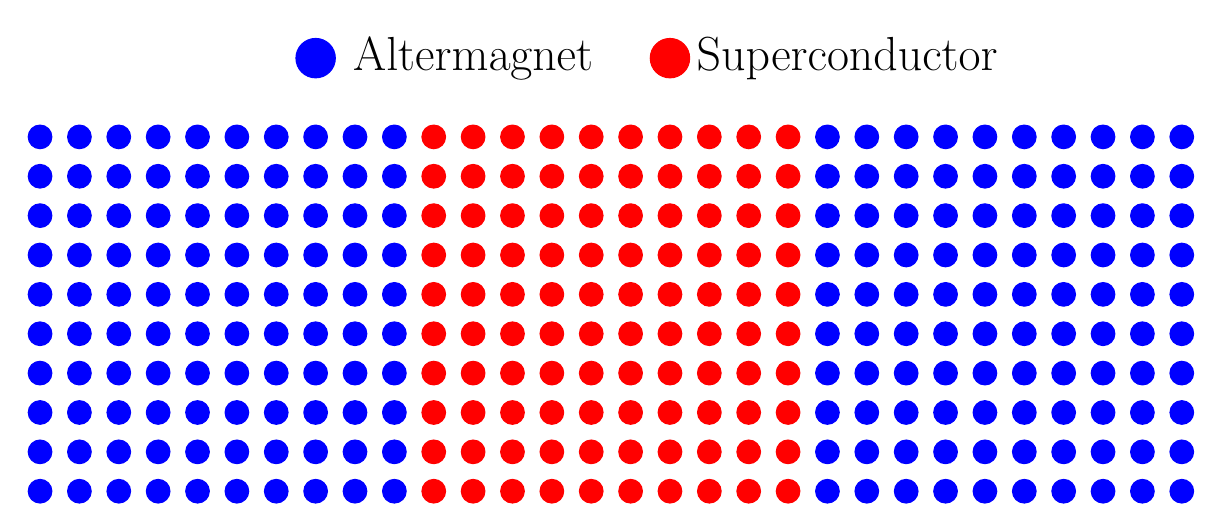
\begin{tikzpicture}[scale=0.5, rotate=0]
    % define lattice parameters
    \def\a{1} 
    % \def\halfa{0.5*\a}
    \filldraw[blue] ({8.},{12}) circle (0.5);
    \node at (12, 12) {\LARGE Altermagnet};

    \filldraw[red] ({17.},{12}) circle (0.5);
    \node at (21.5, 12) {\LARGE Superconductor};

    \foreach \i in {1,...,20} {
      \foreach \j in {1,...,10} {
        \ifnum\i>10 % check if j is greater than 2
            \filldraw[red] ({\i*\a},{\a*\j}) circle (0.3);
        \else
            \filldraw[blue] ({\i*\a},{\a*\j}) circle (0.3);
            \fi
      }
    }
    To include a second AM
    \foreach \i in {21,...,30} {
      \foreach \j in {1,...,10} {
        \pgfmathtruncatemacro\parity{mod(\i,2)}
            \filldraw[blue] ({\i*\a},{\a*\j}) circle (0.3);

      }
    }
  \end{tikzpicture}

\end{document}
